%%%%%%%%%%%%%%%%%%%%%%%%%%%%%%%%%%%%%%
%% Header section of Latex document %%
%%%%%%%%%%%%%%%%%%%%%%%%%%%%%%%%%%%%%%

\documentclass[runningheads,a4paper,11pt]{report}

\usepackage{pgf-umlsd}
\usepackage{listings}
\usepackage{tikz}
\usepackage{pgfplots}
\usepackage{pgfplotstable}
\usepackage[numbers]{natbib}
\usepackage{graphicx}
\usepackage{subcaption}

\usepgfplotslibrary{statistics}


\usepackage[a4paper]{geometry}
\usepackage{t1enc}
\usepackage[utf8]{inputenc}
\usepackage{lmodern}

\usepackage[title,titletoc]{appendix}
\usepackage[section]{placeins}
\usepackage{relsize}

\usepackage[normalem]{ulem} %% Provides underlining.
\usepackage{caption} %% Provides captions.
\usepackage{mdframed} %% Provides frames around text and equations.
\usepackage{tikz-cd} %% Provides diagram drawing environment.
\usepackage{adjustbox} %% Provides additional tools to resize content.
% \usepackage[magyar]{babel} %% Provides foreign language support.

%%%%
%% Provides math related environments and directives.
\usepackage{amssymb}
\usepackage{amsthm}
\usepackage{amsmath}
\usepackage{latexsym}

\usepackage{dsfont}
\usepackage{commath}
\usepackage{bm}

%% See http://tex.stackexchange.com/questions/43835/conflict-between-amsthm-and-some-other-package
\let\proof\relax 
\let\endproof\relax

%%%%
%% Provides table environments and related directives.
\usepackage{array}
\usepackage{tabulary}
\usepackage{tabularx}
\usepackage{multirow}
\usepackage{hhline}
\usepackage{diagbox}

%%%%
%% Provides figure environments and related directives.
\usepackage{graphicx}
\makeatletter
\def\maxwidth#1{\ifdim\Gin@nat@width>#1 #1\else\Gin@nat@width\fi}
\def\maxheight#1{\ifdim\Gin@nat@height>#1 #1\else\Gin@nat@height\fi}
\makeatother

\usepackage{fancyvrb}
\usepackage{rotating}

%%%%
%% Provides environment to display source code.
\usepackage{listings} 
\lstset{ 
    literate=%
        {á}{{\'a}}1
        {é}{{\'e}}1
        {í}{{\'i}}1
        {ó}{{\'o}}1
        {ö}{{\"o}}1
        {ő}{{\H{o}}}1
        {ú}{{\'u}}1
        {ü}{{\"u}}1
        {ű}{{\H{u}}}1
        {Á}{{\'A}}1
        {É}{{\'E}}1
        {Í}{{\'I}}1
        {Ó}{{\'O}}1
        {Ö}{{\"O}}1
        {Ő}{{\H{O}}}1
        {Ú}{{\'U}}1
        {Ü}{{\"U}}1
        {Ű}{{\H{U}}}1
    } %% Customization of listings env., to enable non-English accents.

\lstset{
   frame=single,
   basicstyle=\small,
   language=Erlang,
   numbers=left,
   firstnumber=1,
   numberfirstline=true,
%  basicstyle=\ttfamily,
%  columns=fullflexible,
%   keepspaces=true,
} %% Customization of listings environment


%%%%
%% Provides environment to display pseudocode.
\usepackage{algorithm}% http://ctan.org/pkg/algorithms
\usepackage{algpseudocode}% http://ctan.org/pkg/algorithmicx

\newcommand{\repeatcaption}[2]{%
  \addtocounter{figure}{-1}%
  \renewcommand{\thefigure}{\ref{#1}}%
  \captionsetup{list=no, labelformat=simple, labelsep=colon}%
  \captionof{figure}{#2}%
} %% Customization: Using the same figure twice with no new number. See http://tex.stackexchange.com/a/200229

%%%%
%% Provides directives to display followable URL references.
\usepackage{url}
\usepackage{hyperref}
\hypersetup{
  hidelinks,
  linkbordercolor = {0 0 1},
}

%% Customization: Followable links to appendix references.
\makeatletter
\appto{\appendices}{\def\Hy@chapapp{Appendix}}
\makeatother


%%%%
%% Custom document formatting.

% \renewcommand{\abstract}{ \begin{center}\textbf{Abstract}\end{center}}

\setcounter{tocdepth}{2}

\setlength{\parskip}{\baselineskip}%
\setlength{\parindent}{0pt}%

\makeatletter
\renewcommand\subsection{\@startsection{subsubsection}{3}{\z@}%
                       {-18\p@ \@plus -4\p@ \@minus -4\p@}%
                       {4\p@ \@plus 2\p@ \@minus 2\p@}%
                       {\normalfont\normalsize\bfseries\boldmath
                        \rightskip=\z@ \@plus 8em\pretolerance=10000 }}
\makeatother


%%%%
%% Custom theorem environments.
\newtheorem{mydef}{Definition}
\newtheorem{myexamp}{Example}

%%%%
%% Custom symbol definitions and abbreviations.
\makeatletter
\providecommand{\leadsfrom}{%
  \mathrel{\mathpalette\reflect@squig\relax}%
}
\newcommand{\reflect@squig}[2]{%
  \reflectbox{$\m@th#1\leadsto$}%
}
\makeatother

\renewcommand{\labelitemi}{$\circ$}
\newcommand{\edge}[1]{\stackrel{\bf{#1}}{\rightarrow}}
\newcommand{\ledge}[1]{\stackrel{\bf{#1}}{\leftarrow}}
\newcommand{\rel}[1]{\stackrel{\bf{#1}}{\leadsto}}
\newcommand{\trel}[1]{\stackrel{\bf{#1}}{\leadsto^*}}
\newcommand{\lrel}[1]{\stackrel{\bf{#1}}{\leadsfrom}}

\newcommand{\eqname}[1]{\tag*{#1}}% Tag equation with name

\newcommand{\nv}[0]{node(v)}
\newcommand{\ruleref}[1]{(\S\ref{#1})}
\newcommand{\apxref}[1]{(Appendix \ref{#1}.)}
\newcommand{\apxrefm}[3]{(Appendix \ref{#1}., \ref{#2}. és \ref{#3}.)}


\usepackage[utf8]{inputenc}
\usepackage{enumitem}
\usepackage{hyperref}
\usepackage{bashful}
\usepackage{setspace}
\usepackage{color}
\usepackage{xcolor}

\definecolor{codegreen}{rgb}{0,0.6,0}
\definecolor{codegray}{rgb}{0.2,0.2,0.2}
\definecolor{codeblue}{rgb}{0.0,0,0.62}
\definecolor{backcolour}{rgb}{0.95,0.95,0.95}

\newcommand{\lstbasicfont}{\small\fontfamily{pcr}\selectfont}
\newcommand{\lstcommentstyle}{\color{codegreen}\itshape}

\lstdefinestyle{mystyle}{
    backgroundcolor=\color{backcolour},
    commentstyle=\lstcommentstyle,
    keywordstyle=\color{codeblue}\bfseries,
    %identifierstyle=\color{black},
    identifierstyle=\color{codegray}\bfseries,
    %numberstyle=\tiny\color{codegray},
    stringstyle=\color{purple},
    basicstyle=\lstbasicfont,
    %basicstyle=\small\ttfamily,
    breakatwhitespace=false,
    breaklines=true,
    captionpos=b,
    keepspaces=true,
    %numbers=left,
    %numbersep=5pt,
    showspaces=false,
    showstringspaces=false,
    showtabs=false,
    tabsize=2
}

%% To remove syntax highlighting of Erlang codes
%% uncomment the two commented lines
\lstdefinelanguage{myerlang}[]{erlang}{
  morekeywords={spec,fun,bitstring,orelse,andalso,record,include_lib,begin,end},
  otherkeywords={|,||,<-,->,!,[,],\{,\}},
  deletekeywords={list,ok},
%   identifierstyle=\ttfamily,
%   keywordstyle=\ttfamily
}

\lstset{style=mystyle,
literate=
  {∪}{{$\cup$}}1 {∩}{{$\cap$}}1 {∈}{{$\in$}}1 {⊆}{{$\subseteq$}}1
  {∘}{{$\circ$}}1 {-}{{-}}1 {~}{{\texttildelow}}1 {<}{{<}}1
  {>}{{>}}1
}

%%%%%%%%%%%%%%%%%%%%%%%%%%%%%%%%%%%%
%% Body section of Latex document %%
%%%%%%%%%%%%%%%%%%%%%%%%%%%%%%%%%%%%
\pgfplotsset{compat=1.13}
\begin{document}

% \thispagestyle{empty}
% \begin{center}
% {\Huge TDK dolgozat}\\[0.5cm]
% {\bf Nagy Gergely} \\[1cm]
% \end{center}


\begin{titlepage}
  \noindent
  \begin{minipage}{0.25 \textwidth}
    \includegraphics[height=40mm]{figures/cimer.png}
  \end{minipage}
  \hfill
  \begin{minipage}{0.67 \textwidth}
    \large
    Eötvös Loránd University \\
    Faculty of Informatics \\
    Department of Numerical Analysis \\
    
  \end{minipage}

  \vfill

  \begin{center}
    {\LARGE \bfseries Color image analysis and recognition using Zernike moments} 
    % \\[0.5cm]
    \\[2.0cm]
    {\Large TDK thesis}
    \\[3cm]
    %%\\[6cm]
    \begin{minipage}[t]{0.45 \textwidth}
      \emph{Supervisor:} \\[0.25 \baselineskip]
      {\large Zsolt Németh} \\[0.5 \baselineskip]
      Title title title
    \end{minipage}
    \begin{minipage}[t]{0.45 \textwidth}
      \begin{flushright}
        \emph{Author:} \\[0.25 \baselineskip]
        {\large Gergely Nagy} \\[0.5 \baselineskip]
        Computer Science MSc \\ %% The name of your program
        1\textsuperscript{st} year
      \end{flushright}
    \end{minipage}
  \end{center}

  \vfill

  \begin{center}
    \large Budapest

    % \large Date of closing: 23 May 2019 
  \end{center}
\end{titlepage}

%%%%%%%%%%%%%%%%%%%%%%%%%%%%%%%%%
%% Content sections start here %%

\begin{abstract}
Image moments and moment invariants are widely used for image analysis and pattern recognition. The system of orthogonal Zernike polynomials (defined over the complex unit disc) proved to be a useful basis for series expansions because of certain invariance properties.

Conventionally, for multichannel color images RGB decomposition or grayscale conversion was used. By representing the three basic color channels with quaternions, superior results can be obtained. Previously, rotation, scaling and translation invariant Quaternion Zernike Moment Invariants (QZMIs) have been constructed for use on color images~\cite{qzmi}.

In this thesis we introduce a method of transforming a digital RGB image inside the unit circle onto a discrete orthogonal points system. Using this points system for the discretization of the QZMIs, we have achieved significant improvements in the image recognition and reconstruction capabilities of the method, especially under noisy conditions.

[1] B.J. Chen et al. Quaternion Zernike moments and their invariants for color image analysis and object recognition. Signal Processing 2012;92(2): 308-318.

\end{abstract}

\tableofcontents

\chapter{Introduction}
\label{sec:intro}
Algorithms relying on moment invariants are widely used in applications for pattern matching~\cite{app2}, image recognition~\cite{pattern_recognition}, or to extract useful features from images~\cite{zernike_nn}.

Over the past few decades, many different kinds of moments were defined and tested for single-channel, grayscale images. However, extending these techniques to multichannel color images is an important and generally unresolved problem with numerous potential applications. Conventionally, for color images either RGB decomposition or grayscale conversion was used in order to utilize the methods defined for single-channel images. This often leads to loss of information, for example in the case of grayscale conversion (where the average of the color channels is taken) some important color information can be lost.

More recently, the algebra of quaternions has been used to extend the single-channel methods to color images. For example, quaternion Fourier-Mellin moments have been introduced as an extension of the conventional Fourier-Mellin moments~\cite{qfmm}, as well as the quaternion Zernike moments as an extension of the conventional Zernike moments~\cite{qzm}.

The Zernike functions are a system of orthogonal functions defined over the unit disk by Nobel laureate F. Zernike~\cite{zernike}. Using these functions as a basis for series expansions proved to be useful because of certain inherent invariance properties. Zernike moments, and by extension quaternion Zernike moments are defined by these functions.

Considering a digital image as a discrete sampling of an image function defined over a continuous domain, the need arises to discretize the computation of these moments. One important aspect of the discretization is to preserve the orthogonality over the discrete system in order to avoid redundancy and achieve high robustness with respect to noise.

The conventional method for discretizing quaternion Zernike moments (used by \citeauthor{qzmi}~\cite{qzmi}) consists of uniformly distributed points over the unit disk. This method does not achieve discrete orthogonality thus reducing the robustness of the moments. 

Our goal was to create a system over which the quaternion extension of the Zernike functions is discrete orthogonal and thus improve the robustness of quaternion Zernike moments and to decrease the error introduced by discretization.


\section{Contributions}
In this thesis a new method is proposed for the discretization of quaternion Zernike moments over the unit disk. A point system is constructed on the unit disk, over which the Zernike functions extended to quaternions are discrete orthogonal. 

This new method is compared to the original method of computing quaternion Zernike moment via uniform sampling, used by \citeauthor{qzmi}~\cite{qzmi}, as well as to another recent state-of-the-art method using discrete orthogonal moments based on harmonic trigonometric functions~\cite{LiuAcc}. For the tests, image sets from the Columbia Object Image Library~\cite{coil} and the Amsterdam Library of Object Images~\cite{aloi} were used. 

Besides the theoretical invariance properties of QZMIs, these are also verified empirically. The respective image reconstruction capabilities are compared and we find that the proposed method decreases the error of reconstruction significantly.

The methods are also applied to the recognition of rotated, scaled and translated (RST transformed) images with varying levels of either Gaussian or salt-and-pepper noise. We find that with respect to Gaussian noise the new method achieves significantly better rates of recognition, even for images with high noise values. For salt-and-pepper noise no significant difference can be found between the capabilities of the methods.
Additionally, we also show that by decreasing the number of points used for discretization, the new method is able to achieve similar results as the original method with high number of points, but the computational need to obtain these results is much lower using the new method.

A paper based off the results presented in this thesis was submitted for publication~\cite{signal_proc_manu}.

\section{Structure of the thesis}
This section serves as an overview of the structure of this thesis and contains a short summary of each chapter.

Chapter~\ref{sec:intro} serves as an introduction, where the motivation for this work is described and the contributions featured in this thesis are presented.

Chapter~\ref{sec:background} provides the background for our work. The core concepts, such as (quaternion) Zernike moments and invariants are described in detail. A summary of previous methods for the discretization of quaternion Zernike moments is also given. Finally, some applications relying on Zernike moments are described.

The method we propose for the discretization of Zernike moments is presented in Chapter~\ref{sec:maths}. The construction of a discrete orthogonal point system and the proof of discrete orthogonality is also given.

The different methods and technologies used for the computation of the invariants is shown in Chapter~\ref{sec:implementation}. The computation of the proposed new system is also described.

Chapter~\ref{sec:tests} contains the description of all the tests conducted on the methods, such as image reconstruction or recognition. The results of these tests are evaluated and the original and proposed methods are compared.

Finally, Chapter~\ref{sec:conclusion} summarizes the work and results presented in this thesis. Future development possibilities are also presented.

\chapter{Background}
\label{sec:background}
TODO Background

Image moments in general

Explain Zernike moments

QZMI, QZMRI:
greyscale, color, etc

examples, use cases


\chapter{Math?}

\chapter{Implementation?}
This chapter presents the tools and methods used for implementing a program for calculating the QZMIs of an image using both the conventional and the novel method of discretization.

\section{Programming language and libraries used}
The implementation was created using the Python programming language~\cite{python} and relies on the Numpy~\cite{numpy} and Numba~\cite{numba} libraries to achieve efficient and fast computation of the moment invariants, as well as the Python Imaging Library (PIL, Pillow)~\cite{pil} for image manipulation.
Numpy provided a way to efficiently work with arrays and matrices, as well as the quaternion package, which supports the quaternion data type.

Using the just-in-time compilation (JIT) capabilities of Numba (i.e. the \texttt{@jit} annotation), the computationally heavy parts of the implementation could be made almost as fast and efficient as native code. The disadvantage of using JIT is that it limits the available data types and functions, so in the implementation the use of \texttt{@jit} is kept only to the critical, computationally intensive functions. 

\section{Calculating moments and moment invariants}
\begin{figure}[tbp]
    \centering
        \includegraphics[width=0.5\textwidth]{figures/qzmi_classes.png}
    \caption{The relationships between the classes used to calculate QZMIs and QZMRIs}
    \label{fig:classes}
\end{figure}
To obtain the quaternion Zernike moment invariants (QZMIs) of an image as described in Section~\ref{sec:invariance}, the quaternion Zernike moments (QZMs) must be calculated first. \citeauthor{qzmi}~\cite{qzmi} showed that instead of calculating the QZMs directly by using the algebra of quaternions, it is possible to calculate the real and the imaginary parts of the quaternion-valued QZMs individually by using some linear combination of the real and imaginary parts of the complex-valued, single channel Zernike moments. This means that the single channel Zernike moments have to be calculated for all three of the RGB color channels.
Furthermore, the calculation of the Zernike moments requires the computation of the radial polynomials $R_{n,m}$, introduced in~\eqref{eq:radial_poly}.

To calculate the required values, the following four classes were created, each relying on the next one to perform the computation.
\begin{itemize}
    \item \texttt{QZMI}, for calculating the quaternion Zernike moment invariants
    \item \texttt{ZernikeMomentsColor}, for calculating the quaternion-valued Zernike moments
    \item \texttt{ZernikeMomentsMonochrome}, for calculating the complex-valued, single channel Zernike moments
    \item \texttt{RadialPolynomials}, for calculating the values of the radial polynomials at a given point
\end{itemize}
The relationships between these classes are shown on Figure~\ref{fig:classes}, as well as the \texttt{QZMRI} class, which calculates QZMs, which provide only rotation invariance, needed for some test cases. A description of the algorithms used in these classes and the data stored by them is given below.

Since the work presented in this thesis involves changing the way an image is transformed from image coordinates to polar coordinates inside the unit circle, the classes were made modular with respect to the transformation used. This makes it easy to create and test a new image transformation function with the interface expected by the calculating classes.

\subsection{Radial polynomials}
To calculate the value of all $R_{n,m}$ radial polynomials up to some maximal degree $P$ at a point $r \in [0,1]$, the modified Kintner's method was used, as described in~\cite{kintner}. This recursive algorithm computes the value of $R_{n,m}(r)$ for all $0 \leq |m| \leq n \leq P$, ($n - |m|$ is even) with complexity $\mathcal{O}(P^2)$. Note that Kintner's method is ideal for the precomputation of all radial polynomial values up to a maximum degree.


The modified Kintner's method utilizes the recurrence relation
\begin{gather*}
    R_{n,m}(r) =  \frac{(K_2r^2 + K_3)R_{n-2,m}(r) + K_4R_{n-4,m}(r)}{K_1},
\end{gather*}
where $n \neq m$ and $n - m \neq 2$, and the coefficients $K_i, \ i = 1,2,3,4$ are defined as
\begin{gather*}
    \begin{split}
        K_1 &= \frac{(n + m)(n - m)(n - 2)}{2}\\
        K_2 &= 2n(n-1)(n-2)\\
        K_3 &= -m^2(n-1)-n(n-1)(n-2)\\
        K_4 &= \frac{-n(n + m - 2)(n - m - 2)}{2}.
    \end{split}
\end{gather*}
In the cases where $n = m$ or $ n - m = 2$ the following formulas can be used:
\begin{gather*}
    \begin{split}
        R_{n,n}(r) &= r^n\\
        R_{n,n - 2}(r) &= nR_{n,n}(r) - (n - 1)R_{n-2,n-2}(r).
    \end{split}
\end{gather*}


Since this routine is called many times during the calculation of Zernike moments, just-in-time compilation was used to further increase efficiency. Figure~\ref{fig:radial_code} shows the JIT-enabled function.

\begin{figure}[tbp]
    \centering
    \begin{lstlisting}[language=Python]
@jit(void(float64, int32, float64[:,:]), nopython=True)
def calculateRadialPolynomials(r, P, values):
  values[0,0] = 1
  values[1,1] = r
  for n in range(2,P + 1):
    h = n*(n - 1)*(n - 2)
    K2 = 2*h
    values[n,n] = (r**n)
    values[n,n-2] = n*values[n,n] - (n-1)*values[n-2,n-2]
    for m in range(n-4,-1,-2):			
      K1 = (n + m)*(n - m)*(n - 2)/2
      K3 = (-1)*m*m*(n - 1) - h
      K4 = (-1)*n*(n + m - 2)*(n - m - 2)/2
      r2 = r**2
      values[n,m] = ((K2*r2+K3)*values[n-2,m]+K4*values[n-4,m])/K1\end{lstlisting}
    \caption{Function for calculating radial polynomial values}
    \label{fig:radial_code}
\end{figure}

\subsection{Complex Zernike moments}
The \texttt{ZernikeMomentsMonochrome} class calculates the conventional Zernike moments of degree at most $P$ of a square $N \times N$, single channel (grayscale) image. The algorithm is based directly on the discretized definition of the Zernike moments.
For the original linear transformation of the image onto the unit disk, this gives:
\begin{gather*}
    \begin{split}
    Z_{n,m}(f) &= \lambda\frac{(n+1)}{(N-1)^2}\sum_{x=1}^{N}\sum_{y=1}^{N}f(x,y)V_{n,m}^{*}(r_{x,y},\theta_{x,y}) \\
    &= \lambda\frac{(n+1)}{(N-1)^2}\sum_{x=1}^{N}\sum_{y=1}^{N}f(x,y)R_{n,m}(r_{x,y})e^{-\bm{i}m\theta_{x,y}} \\
    &= \lambda\frac{(n+1)}{(N-1)^2}\sum_{x=1}^{N}\sum_{y=1}^{N}f(x,y)R_{n,m}(r_{x,y})(\cos (m\theta_{x,y}) - \bm{i}\sin (m\theta_{x,y})),
    \end{split}
\end{gather*}
where $0\leq |m| \leq n \leq P$, $n - |m|$ is even, $(r_{x,y},\theta_{x,y})$ are the polar form of the $(x,y)$ coordinates transformed to the unit disk, $\lambda$ is the scaling parameter also given by the transformation (as described in Section~\ref{sec:discretization}) and $f$ is the real-valued, grayscale image.

Precomputing the sine and cosine values for all possible combinations of $m$ and $\theta_{x,y}$, as well as precomputing the values of the radial polynomials, this formula gives an efficient way to calculate the real and imaginary parts of the Zernike moments separately. This way only primitive data types have to be used during the computation, hence it can be made more efficient using JIT.

Also, there is no need to calculate the Zernike moments for $m < 0$ values, as the $Z_{n,m}(f) = Z_{n,-m}(f)^{*}$ identity can be used later to obtain the values for $m < 0$.

\subsection{Quaternion Zernike moments}
The class \texttt{ZernikeMomentsColor} calculates the quaternion Zernike moments of an RGB image. First, the conventional Zernike moments for each of the three color channels are calculated, then the relationship between QZMs and Zernike moments is applied to construct the quaternions~\cite{qzmi}:
\begin{gather}
    \begin{split}
        Z_{n,m}^R(f) = &-\frac{1}{\sqrt{3}}\left( \ip(Z_{n,m}(f_R)) + \ip(Z_{n,m}(f_G)) + \ip(Z_{n,m}(f_B)) \right)\\
        &+\left[\rp(Z_{n,m}(f_R)) + \frac{1}{\sqrt{3}}\left(\ip(Z_{n,m}(f_G)) - \ip(Z_{n,m}(f_B))\right)\right]\bm{i}\\
        &+\left[\rp(Z_{n,m}(f_G)) + \frac{1}{\sqrt{3}}\left(\ip(Z_{n,m}(f_B)) - \ip(Z_{n,m}(f_R))\right)\right]\bm{j}\\
        &+\left[\rp(Z_{n,m}(f_B)) + \frac{1}{\sqrt{3}}\left(\ip(Z_{n,m}(f_R)) - \ip(Z_{n,m}(f_G))\right)\right]\bm{k},\\
    \end{split} \label{eq:QZM_ZM}
\end{gather}
where $f$ is an RGB image, $f_R, f_G, f_B$ are the red, green and blue color channels respectively and $Z_{n,m}^R$ denote the right-side quaternion Zernike moments, while $Z_{n,n}$ denote the conventional Zernike moments. 

Again, only the QZMs $Z_{n,m}^R$ ($m \geq 0$) are calculated, because for $m < 0$ the $Z_{n,m}^R(f) = Z_{n,-m}^R(f)^{*}$ equality can be used.

\subsection{Invariants}
The class \texttt{QZMI} is responsible for computing the combined rotation, scaling and translation (RST) invariant moments, while the class \texttt{QZMRI} computes the moments which are invariant only to rotation.
The invariants for scaling and rotation are calculated directly using the QZMs, based on the formulas described in Section~\ref{sec:invariance}.

To achieve translation invariance, the common centroid (introduced in \eqref{eq:common_centroid}) of the RGB image is calculated based on the formulas described by ~\citeauthor{affine_color}~\cite{affine_color}.
\begin{gather*}
    \left\{x_c,y_c\right\} = \left\{\frac{M_{10}(f_R)+M_{10}(f_G)+M_{10}(f_B)}{M_{00}(f_R)+M_{00}(f_G)+M_{00}(f_B)}, \frac{M_{01}(f_R)+M_{01}(f_G)+M_{01}(f_B)}{M_{00}(f_R)+M_{00}(f_G)+M_{00}(f_B)}\right\},
\end{gather*}
where $f_R, f_G, f_B$ are the grayscale images corresponding to the red, green and blue color channels respectively, and $M_{10}, M_{01}, M_{00}$ are the regular image moments introduced in~\eqref{eq:regular_moment}.
The original image $f$ is then translated in image coordinates such that the origin falls on the common centroid $\{x_c,y_c\}$, and later on scaling and rotation invariants are calculated based on this translated image.


\subsection{Quaternion radial harmonic Fourier moments}
QRHFMs can be calculated using the conventional radial harmonic Fourier moments. This is achieved using a similar formula to the one in \eqref{eq:QZM_ZM}.

As described in Section~\ref{sec:invariance}, rotation invariants can be constructed by taking modulus of each moment (as used by \citeauthor{LiuAcc}~\cite{LiuAcc}).
However, in order to ensure fair comparison between the capabilities of QZMs and QRHFMs, we construct rotation invariants in a similar way to the construction in \eqref{eq:rot_inv} for QZMs.

By calculating the product of left- and right-side QRHFMs we get quaternion-valued invariants instead of real-valued invariants. This construction provides rotation invariance, while ensuring that any difference in the capabilities of the methods does not originate from the difference in the construction of the invariants.

We also remark that in our experiments, instead of relying on fast Fourier transform (FFT), we utilized a direct computation of radial harmonic Fourier moments. Theoretically, this can end up being a slightly slower method for large image dimensions, but provides more stable numeric results.

\section{New image transformation}\label{sec:new_trans}
The new image transformation, as described in Chapter~\ref{sec:maths}, requires the calculation of the roots of the $n^{th}$ degree Legendre polynomials $P_n$, as well as calculating the integrals of the Lagrange basis polynomials over the roots of $P_n$. Furthermore, since when applying the linear transformation from image coordinates to polar coordinates, the pixels of the image do not fall exactly on any point of the new discrete point system, some interpolating methods have to be used to approximate the image values at these points.

Because of the modularity of the previously described classes, it is possible to swap the old transformation with the new one. With some minor modifications during the calculation of the conventional Zernike moments -- because of the new discretization formula containing a different measure -- the previous classes can be used to obtain the QZMIs using the new method of discretization.

\subsection{Roots of Legendre polynomials}
The roots of the Legendre polynomial $P_n$ are essential for the calculation of the new point system. An explicit formula for the roots does not exist, thus an efficient and fast iterative algorithm is utilized to calculate these roots.

The $n^{th}$ degree Legendre polynomial $P_n$ satisfies the following differential equation:
\begin{gather}
    (1-x^2)P_n''(x) - 2xP_n'(x) + n(n+1)P_n(x) = 0.\label{eq:legendre_de}
\end{gather}
A fast algorithm for calculating the roots of $P_n$, based on this differential equation was presented by \citeauthor{legendre_algo}~\cite{legendre_algo}. The algorithm uses a second-order Runge-Kutta method (namely the midpoint method) to solve \eqref{eq:legendre_de} for some given initial condition. A first approximation for a root of $P_n$ can be obtained from the solution of the initial value problem. This approximation is then further refined by Newton's method.
Subsequent roots can be calculated using the same method but starting from different initial conditions defined by the previous root.

In practice, this algorithm calculates the roots of $P_n$ with accuracy up to machine precision in only just a few, predefined number of iterations for both the Runge-Kutta and the Newton's method.

\subsection{Computing the discrete measure}
To calculate the Zernike moments over the discrete orthogonal point system, apart from the $\lambda_{n,m} = n + 1$ scaling factor, a weight function is used as well (as described in \eqref{eq:QZMappr}). To calculate these $w(r_{k,N},\theta_{j,N})$ weight values (defined in \eqref{weight}), the following integral has to be calculated:
\begin{gather*}
    \mathcal{A}_{k,N} = \int_{-1}^{1}\ell_{k,N}(x)\ dx,
\end{gather*}
where $\ell_{k,N}$ is the $k^{th}$ Lagrange basis polynomial corresponding to the roots of the Legendre polynomial $P_N$, meaning that
\begin{gather*}
    \ell_{k,N}(x) = \frac{(x - x_1)(x - x_2)\ldots(x - x_{k-1})(x - x_{k+1})\ldots(x - x_{N-1})(x - x_N)}{(x_k - x_1)(x_k - x_2)\ldots(x_k - x_{k-1})(x_k - x_{k+1})\ldots(x_k - x_{N-1})(x_k - x_N)},
\end{gather*}
where $x_i, \ i = 1,\ldots,N$ are the roots of $P_N$.

The Gauss-Legendre quadrature is a numerical method used for approximating the definite integral of a function over the interval $[-1,1]$. This method is based on the roots of the Legendre polynomial $P_n$ of degree $n$. Let $x_1,x_2,\ldots,x_n$ denote the roots of $P_n$. The quadrature provides the following approximation of a definite integral:
\begin{gather*}
    \int_{-1}^{1}f(x)\ dx \approx \sum_{k=1}^n w_k f(x_k), \\
    w_k = \frac{2}{(1-x_k^2)(P_n'(x_k))^2}.
\end{gather*}
The quadrature is exact for all polynomials whose degree is at most $2n-1$. Now $\ell_{k,N}(x)$ is an $N-1$ degree polynomial, so the Gauss-Legendre quadrature with $n=N$ is exact for $\ell_{k,N}$. Furthermore, $\ell_{k,N}$ is defined such that $\ell_{k,N}(x_i) = 0$ for $i \neq k$, and $\ell_{k,N}(x_k) = 1$ Thus:
\begin{gather*}
    \int_{-1}^{1}\ell_{k,N}(x)\ dx = w_k = \frac{2}{(1-x_k^2)(P_n'(x_k))^2}.
\end{gather*}

Since the roots of the Legendre polynomial $P_N$ must be computed to obtain the point system, this formula gives an easy and fast way to calculate the exact values of the weight function $w$.


Additionally, the values of the derivative $P'_n$ are needed at the point $x_k$. For this the recurrence relations presented by \citeauthor{legendre_algo}~\cite{legendre_algo} are used:
\begin{gather*}
    \begin{split}
        P_{n+1}(x) &= \frac{2n + 1}{n + 1}xP_n(x) - \frac{n}{n + 1}P_{n-1}(x)\\
        P'_{n+1}(x) &= \frac{2n + 1}{n + 1}(xP'_n(x) + P_n(x)) - \frac{n}{n+1}P'_{n-1},
    \end{split}
\end{gather*}
with the initial values of $P_{-1}(x) = P'_{-1}(x) = P'_0(x) = 0$ and $P_0(x) = 1$.

\subsection{Image interpolation}
After obtaining the discrete orthogonal point system, the values of the image function have to be approximated at each point, because the original pixel values do not fall exactly on the new points. Now we describe some reasonable ways of resampling the image data to fit these new points.

First, the image is linearly transformed onto the unit disk using the transformation shown on Figure~\ref{fig:transform2}, so that the the transformed image covers the entire unit disk. This transformation is used as opposed to the one on Figure~\ref{fig:transform1}, because the point system covers the entire unit disk, so the image also has to cover the whole disk.

There are two ways to approximate the values at each point, depending on the number of points in the discrete orthogonal point system.

\paragraph{Approximately the same number of points as pixels.}
If the number of points is approximately the same as the number of pixels in the image, then bilinear interpolation can be used for each point.

First, the four pixels of the image that are closest to the given point $(x,y)$ are determined. These four points form a square. Then, the weighted average of these points is calculated along the $x$ axis, giving approximate function values at two points, which only differ in their $y$ coordinate. Finally, the weighted average of the function values at these points is calculated to get the approximation of $f(x,y)$. The points involved in this interpolation are shown on Figure~\ref{fig:bilinear}.

\begin{figure}[tb]
    \centering
    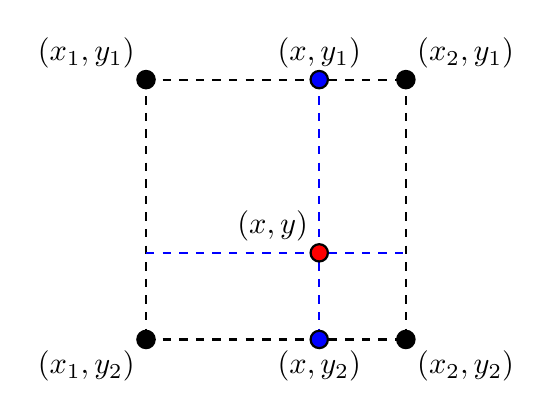
\begin{tikzpicture}[thick,scale=1.1, every node/.style={transform shape}]
        \draw[thick,dashed] (-2,2) -- (1,2);
        \draw[thick,dashed] (-2,2) -- (-2,-1);
        \draw[thick,dashed] (1,2) -- (1,-1);
        \draw[thick,dashed] (-2,-1) -- (1,-1);
        \draw[fill] (-2,2) circle (0.1) node[anchor=south east] {$(x_1,y_1)$};
        \draw[fill] (1,2) circle (0.1) node[anchor=south west] {$(x_2,y_1)$};
        \draw[fill] (-2,-1) circle (0.1) node[anchor=north east] {$(x_1,y_2)$};
        \draw[fill] (1,-1) circle (0.1) node[anchor=north west] {$(x_2,y_2)$};
        
        \draw[thick,blue,dashed] (0,2) -- (0,-1);
        \draw[thick,blue,dashed] (-2,0) -- (1,0);
        \draw[fill=red] (0,0) circle (0.1) node[anchor=south east] {$(x,y)$};
        \draw[fill=blue] (0,2) circle (0.1) node[anchor=south] {$(x,y_1)$};
        \draw[fill=blue] (0,-1) circle (0.1) node[anchor=north] {$(x,y_2)$};
    \end{tikzpicture}

    \caption{The point $(x,y)$ and its neighboring points, which are used to approximate $f(x,y)$ by bilinear interpolation}
    \label{fig:bilinear}
\end{figure}

\paragraph{Much fewer points than the number of pixels.}
If the number of points is far below the number of pixels, then many of the original pixel values would not be represented in the final approximate function values when using bilinear interpolation. Therefore, the following algorithm is used to approximate function values using discrete integration.

First, assign each pixel of the original image to the point which is the closest to it in the discrete orthogonal system. This results in a set of pixels assigned to each point. Then, for each point in the discrete orthogonal point system, calculate the average of this set of pixels. This algorithm divides the unit disk into annular sections based on proximity to the new points, meaning that the set of pixels belonging to a point form annular sections. This is shown on Figure~\ref{fig:interpolation_integral}.

The comparison between one of the original transformations and the two methods for approximating function values is shown on Figure~\ref{fig:pepper_trans} on the peppers image from the USC-SIPI Image Database~\cite{usc_sipi}.

\begin{figure}[tb]
    \begin{subfigure}{.45\textwidth}
    \centering
    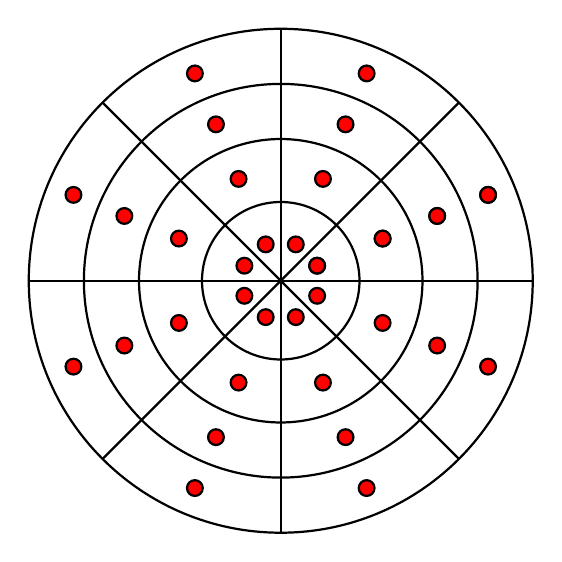
\begin{tikzpicture}[thick,scale=1, every node/.style={transform shape}]
        \foreach \r in {1,1.8,2.5,3.2}
            \draw (0,0) circle (\r);
        \foreach \x in {0,45,...,360} {
            \draw[thick] (0,0) -- (\x:3.2);
            \foreach \r in {0.5,1.4,2.15,2.85}
                \draw[fill=red] (22.5+\x:\r) circle (0.1);
        }
    \end{tikzpicture}

    \caption{The point system on the unit disk and the annular sectors over which the pixel values are averaged.}
    \end{subfigure}
    \hspace{.05\textwidth}
    \begin{subfigure}{.45\textwidth}
        \centering
        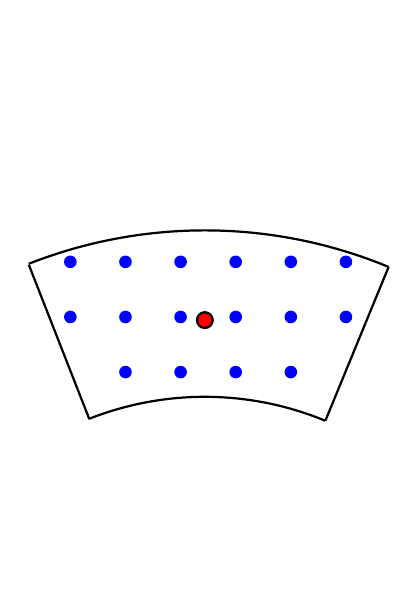
\begin{tikzpicture}[thick,scale=1, every node/.style={transform shape}]
            \draw (6.1*0.3826,6.1*0.9304) arc (67.5:111.5:6.1);
            \draw (4*0.3826,4*0.9304) arc (67.5:111.5:4);
            \draw (4*0.3826,4*0.9304) -- (6.1*0.3826,6.1*0.9304);
            \draw (-4*0.3665,4*0.935) -- (-6.1*0.3665,6.1*0.935);
            \foreach \x in {0,1,...,3} {
                \foreach \y in {2,3,...,4} {
                    \fill[color=blue] (0.7*\x-0.7*1.44,0.7*\y+0.7*4.2) circle (0.08);
                }
            }
            \fill[color=blue] (-0.7-0.7*1.44,0.7*3+0.7*4.2) circle (0.08);
            \fill[color=blue] (-0.7-0.7*1.44,0.7*4+0.7*4.2) circle (0.08);
            \fill[color=blue] (4*0.7-0.7*1.44,0.7*3+0.7*4.2) circle (0.08);
            \fill[color=blue] (4*0.7-0.7*1.44,0.7*4+0.7*4.2) circle (0.08);
            \draw[fill=red] (90:5) circle (0.1);
            \draw[color=white] (0,2) circle (0.1);
            \draw[color=white] (0,8.60) circle (0.1);
        \end{tikzpicture}
    
        \caption{A single annular sector with the original image pixels (blue) and the point in which the approximate function value has to be calculated (red).}
        \end{subfigure}
        \caption{}
    \label{fig:interpolation_integral}
\end{figure}


\begin{figure}[tbh]
    \centering
    \begin{subfigure}{.49\textwidth}
        \centering
    \includegraphics[width=\textwidth]{figures/pepper_color_256.png}
    \caption{Original image}
    \end{subfigure}
    \begin{subfigure}{.49\textwidth}
        \centering
    \includegraphics[width=\textwidth]{figures/pepper_square.png}
    \caption{Original transformation}
    \end{subfigure}
    \begin{subfigure}{.49\textwidth}
        \centering
    \includegraphics[width=\textwidth]{figures/pepper_bilinear.png}
    \caption{Bilinear interpolation}
    \end{subfigure}
    \begin{subfigure}{.49\textwidth}
        \centering
    \includegraphics[width=\textwidth]{figures/pepper_integral.png}
    \caption{Interpolation by integrals}
    \end{subfigure}
    \caption{Different transformations with different interpolation methods of the peppers image.}
    \label{fig:pepper_trans}
\end{figure}

\chapter{Tests/improvements?}
In this chapter we present the different tests that were performed to compare the capabilities of the old and new methods. For each test, the results of both methods of discretization are compared.

In total, four kinds of tests were conducted:
\begin{itemize}
	\item Invariance
	\item Image reconstruction
	\item Image recognition
	\item Template matching
\end{itemize}

\section{Test images}\label{sec:test_images}
The images for testing were acquired from multiple online image libraries. The Lenna and Pepper images~\cite{usc_sipi} (shown on Figure~\ref{fig:lena_pepper_original}) were used to test image reconstruction as well as to demonstrate the different points systems.

\begin{figure}[tbp]
    \begin{subfigure}{0.49\textwidth}
        \centering
    \includegraphics[width=128pt]{figures/lenna_color_256.png}
    \caption{}
	\end{subfigure}
	\begin{subfigure}{0.49\textwidth}
        \centering
    \includegraphics[width=128pt]{figures/pepper_color_256.png}
    \caption{}
	\end{subfigure}
	\caption{The Lenna and Pepper images}
	\label{fig:lena_pepper_original}
\end{figure}

For the image recognition tests, two sets of images were used. The first set consists of 14 images chosen from the Columbia Object Image Library (COIL-100)~\cite{coil}, shown on Figure~\ref{fig:coil_original}. These images are originally $128 \times 128$ pixels, but they were placed on a $204 \times 204$ black background so that the rotated, scaled and translated versions of the images remain completely within these dimensions. 

A set of 1008 rotated images was created by rotating each of the 14 images by a degree $\alpha\in\{0,5,10,\ldots,350,355\}$. Some examples of the extended and rotated images are shown on Figure~\ref{fig:coil_rot}.

Another set of 1176 rotated, scaled and translated images was created by translating each image by -11 pixels in the $x$ direction and 9 pixels in the $y$ direction. Then the translated images were rotated by $\alpha \in \{0,30,60,\ldots,300,330\}$. Finally, each rotated and translated image was scaled by $\lambda \in \{0.5, 0.75, \ldots, 1.75, 2\}$. Some examples of the RST transformed images are shown on Figure~\ref{fig:coil_rst}.

\begin{figure}[tbp]
    \begin{subfigure}{80pt}
        \centering
    \includegraphics[width=\textwidth]{figures/coil_original/7.png}
    \caption{}
	\end{subfigure}
	\begin{subfigure}{80pt}
        \centering
    \includegraphics[width=\textwidth]{figures/coil_original/13.png}
    \caption{}
	\end{subfigure}
	\begin{subfigure}{80pt}
        \centering
    \includegraphics[width=\textwidth]{figures/coil_original/22.png}
    \caption{}
	\end{subfigure}
	\begin{subfigure}{80pt}
        \centering
    \includegraphics[width=\textwidth]{figures/coil_original/26.png}
    \caption{}
	\end{subfigure}
	\begin{subfigure}{80pt}
        \centering
    \includegraphics[width=\textwidth]{figures/coil_original/29.png}
    \caption{}
	\end{subfigure}
	\begin{subfigure}{80pt}
        \centering
    \includegraphics[width=\textwidth]{figures/coil_original/32.png}
    \caption{}
	\end{subfigure}
	\begin{subfigure}{80pt}
        \centering
    \includegraphics[width=\textwidth]{figures/coil_original/39.png}
    \caption{}
	\end{subfigure}
	\begin{subfigure}{80pt}
        \centering
    \includegraphics[width=\textwidth]{figures/coil_original/55.png}
    \caption{}
	\end{subfigure}
	\begin{subfigure}{80pt}
        \centering
    \includegraphics[width=\textwidth]{figures/coil_original/62.png}
    \caption{}
	\end{subfigure}
	\begin{subfigure}{80pt}
        \centering
    \includegraphics[width=\textwidth]{figures/coil_original/64.png}
    \caption{}
	\end{subfigure}
	\begin{subfigure}{80pt}
        \centering
    \includegraphics[width=\textwidth]{figures/coil_original/65.png}
    \caption{}
	\end{subfigure}
	\begin{subfigure}{80pt}
        \centering
    \includegraphics[width=\textwidth]{figures/coil_original/71.png}
    \caption{}
	\end{subfigure}
	\begin{subfigure}{80pt}
        \centering
    \includegraphics[width=\textwidth]{figures/coil_original/95.png}
    \caption{}
	\end{subfigure}
	\begin{subfigure}{80pt}
        \centering
    \includegraphics[width=\textwidth]{figures/coil_original/99.png}
    \caption{}
    \end{subfigure}
	\caption{The 14 selected images from the Columbia Object Image Library (COIL-100)}
	\label{fig:coil_original}
\end{figure}

\begin{figure}[tbp]
	\begin{subfigure}{0.30\textwidth}
        \centering
    \includegraphics[width=102pt]{figures/coil_rot/7r0.png}
    \caption{$\alpha=0^{\circ}$}
	\end{subfigure}
	\begin{subfigure}{0.30\textwidth}
        \centering
    \includegraphics[width=102pt]{figures/coil_rot/7r35.png}
    \caption{$\alpha=35^{\circ}$}
	\end{subfigure}
	\begin{subfigure}{0.30\textwidth}
        \centering
    \includegraphics[width=102pt]{figures/coil_rot/7r255.png}
    \caption{$\alpha=255^{\circ}$}
	\end{subfigure}
	\caption{Some extended and rotated images from COIL}
	\label{fig:coil_rot}
\end{figure}

\begin{figure}[tbp]
	\begin{subfigure}{0.30\textwidth}
        \centering
    \includegraphics[width=102pt]{figures/coil_rst/26x-11y9r0s1_0.png}
    \caption{$\alpha=0^{\circ}$, $\lambda=1$}
	\end{subfigure}
	\begin{subfigure}{0.29\textwidth}
        \centering
    \includegraphics[width=51pt]{figures/coil_rst/26x-11y9r150s0_5.png}
    \caption{$\alpha=150^{\circ}$, $\lambda=0.5$}
	\end{subfigure}
	\begin{subfigure}{0.40\textwidth}
        \centering
    \includegraphics[width=153pt]{figures/coil_rst/26x-11y9r270s1_75.png}
    \caption{$\alpha=270^{\circ}$, $\lambda=1.5$}
	\end{subfigure}
	\caption{Some RST transformed images from COIL. All images are translated by $\Delta x = -11$, $\Delta y = 9$}
	\label{fig:coil_rst}
\end{figure}

Another set of 13 images was acquired from the Amsterdam Library of Object Images (ALOI)~\cite{aloi}. These are shown on Figure~\ref{fig:aloi_original}. Originally, these size of these images was $768 \times 576$ pixels, but the were downscaled to $96 \times 72$ and subsequently extended to $152 \times 128$ by placing the images on a black background. Similarly to the test sets created using the COIL-100 images, the ALOI images were also translated, rotated and scaled, yielding a set of 1092 RST transformed images. The parameters of the transformation were the same as for the COIL-100 images, except for the translation, where $\Delta x = 8$ and $\Delta y = 5$ was used.

\begin{figure}[tbp]
    \begin{subfigure}{80pt}
        \centering
    \includegraphics[width=\textwidth]{figures/aloi_original/36.png}
    \caption{}
	\end{subfigure}
	\begin{subfigure}{80pt}
        \centering
    \includegraphics[width=\textwidth]{figures/aloi_original/125.png}
    \caption{}
	\end{subfigure}
	\begin{subfigure}{80pt}
        \centering
    \includegraphics[width=\textwidth]{figures/aloi_original/127.png}
    \caption{}
	\end{subfigure}
	\begin{subfigure}{80pt}
        \centering
    \includegraphics[width=\textwidth]{figures/aloi_original/153.png}
    \caption{}
	\end{subfigure}
	\begin{subfigure}{80pt}
        \centering
    \includegraphics[width=\textwidth]{figures/aloi_original/157.png}
    \caption{}
	\end{subfigure}
	\begin{subfigure}{80pt}
        \centering
    \includegraphics[width=\textwidth]{figures/aloi_original/161.png}
    \caption{}
	\end{subfigure}
	\begin{subfigure}{80pt}
        \centering
    \includegraphics[width=\textwidth]{figures/aloi_original/259.png}
    \caption{}
	\end{subfigure}
	\begin{subfigure}{80pt}
        \centering
    \includegraphics[width=\textwidth]{figures/aloi_original/262.png}
    \caption{}
	\end{subfigure}
	\begin{subfigure}{80pt}
        \centering
    \includegraphics[width=\textwidth]{figures/aloi_original/308.png}
    \caption{}
	\end{subfigure}
	\begin{subfigure}{80pt}
        \centering
    \includegraphics[width=\textwidth]{figures/aloi_original/507.png}
    \caption{}
	\end{subfigure}
	\begin{subfigure}{80pt}
        \centering
    \includegraphics[width=\textwidth]{figures/aloi_original/514.png}
    \caption{}
	\end{subfigure}
	\begin{subfigure}{80pt}
        \centering
    \includegraphics[width=\textwidth]{figures/aloi_original/774.png}
    \caption{}
	\end{subfigure}
	\begin{subfigure}{80pt}
        \centering
    \includegraphics[width=\textwidth]{figures/aloi_original/875.png}
    \caption{}
	\end{subfigure}
	\caption{The 13 selected images from the Amsterdam Library of Object Images (ALOI)}
	\label{fig:aloi_original}

\end{figure}

\section{Invariance test}
In order to test the invariance of the quaternion Zernike moment invariants with respect to rotation, scaling and translation, the QZMIs of order 1 to 4 were calculated for a given image and all of its RST transformations. Then, the modulus of these QZMIs was calculated, as well as the mean ($\mu$), standard deviation ($\sigma$) and $\frac{\sigma}{\mu}$ for the same moment of all transformed images.

\subsection{Results}
The modulus of the QZMIs for the transformed images shown on Figure %TODO: make figure
is shown in Table~\ref{tab:inv_old} for the old method of discretization and in Table~\ref{tab:inv_new} for the new, proposed method of discretization. The coefficient of variation ($\frac{\sigma}{\mu}$) shows that using both methods, the moments are invariant to RST transformation, but comparing the two methods, the proposed one yields slightly lower coefficient of variation for most moments.

\begin{table}
	\centering
\begin{tabular}{| c || c | c | c | c | c | c || c | } \hline
& a & b & c & d & e & f & $\frac{\sigma}{\mu}$ \\ \hline\hline
$|\overline{\Psi}_{1,1}^1|$ & a & b & c & d & e & f & g \\ \hline
$|\overline{\Psi}_{2,0}^0|$ & a & b & c & d & e & f & g \\ \hline
$|\overline{\Psi}_{2,2}^0|$ & a & b & c & d & e & f & g \\ \hline
$|\overline{\Psi}_{2,2}^2|$ & a & b & c & d & e & f & g \\ \hline
$|\overline{\Psi}_{3,1}^1|$ & a & b & c & d & e & f & g \\ \hline
$|\overline{\Psi}_{3,3}^1|$ & a & b & c & d & e & f & g \\ \hline
$|\overline{\Psi}_{3,3}^3|$ & a & b & c & d & e & f & g \\ \hline
$|\overline{\Psi}_{4,0}^0|$ & a & b & c & d & e & f & g \\ \hline
$|\overline{\Psi}_{4,2}^0|$ & a & b & c & d & e & f & g \\ \hline
$|\overline{\Psi}_{4,2}^2|$ & a & b & c & d & e & f & g \\ \hline
$|\overline{\Psi}_{4,4}^0|$ & a & b & c & d & e & f & g \\ \hline
$|\overline{\Psi}_{4,4}^2|$ & a & b & c & d & e & f & g \\ \hline
$|\overline{\Psi}_{4,4}^4|$ & a & b & c & d & e & f & g \\ \hline
\end{tabular}
\caption{The modulus of QZMIs using the old method for discretization. Note that $\frac{\sigma}{\mu}$ was calculated using the QZMIs for all transformation of the image, not juts the values shown in the table.}
\label{tab:inv_old}
\end{table} % TODO fill out table based on original_inv.csv

\begin{table}
	\centering
\begin{tabular}{| c || c | c | c | c | c | c || c | } \hline
& a & b & c & d & e & f & $\frac{\sigma}{\mu}$ \\ \hline\hline
$|\overline{\Psi}_{1,1}^1|$ & a & b & c & d & e & f & g \\ \hline
$|\overline{\Psi}_{2,0}^0|$ & a & b & c & d & e & f & g \\ \hline
$|\overline{\Psi}_{2,2}^0|$ & a & b & c & d & e & f & g \\ \hline
$|\overline{\Psi}_{2,2}^2|$ & a & b & c & d & e & f & g \\ \hline
$|\overline{\Psi}_{3,1}^1|$ & a & b & c & d & e & f & g \\ \hline
$|\overline{\Psi}_{3,3}^1|$ & a & b & c & d & e & f & g \\ \hline
$|\overline{\Psi}_{3,3}^3|$ & a & b & c & d & e & f & g \\ \hline
$|\overline{\Psi}_{4,0}^0|$ & a & b & c & d & e & f & g \\ \hline
$|\overline{\Psi}_{4,2}^0|$ & a & b & c & d & e & f & g \\ \hline
$|\overline{\Psi}_{4,2}^2|$ & a & b & c & d & e & f & g \\ \hline
$|\overline{\Psi}_{4,4}^0|$ & a & b & c & d & e & f & g \\ \hline
$|\overline{\Psi}_{4,4}^2|$ & a & b & c & d & e & f & g \\ \hline
$|\overline{\Psi}_{4,4}^4|$ & a & b & c & d & e & f & g \\ \hline
\end{tabular}
\caption{The modulus of QZMIs using the new method for discretization. Note that $\frac{\sigma}{\mu}$ was calculated using the QZMIs for all transformation of the image, not juts the values shown in the table.}
\label{tab:inv_new}
\end{table} % TODO fill out table based on leg_inv.csv

\section{Image reconstruction}

\section{Image recognition}

\section{Template matching}


\chapter{Conclusion}
\label{sec:conclusion}
In this chapter we summarize the work and results presented in this thesis. We also present a short overview of further possibilities based on this work.

We have constructed a points system on the unit disk, over which the quaternion extension of the Zernike functions is discrete orthogonal. Using this method of discretization, the quaternion Zernike moments are more robust to noise than with the previously used method.

Many tests have been performed on large sets of images to verify and quantify the improvements of the method.
First, the invariance properties of the QZMIs have been verified empirically using the proposed method.

By comparing the image reconstruction capabilities of the original and the proposed method, we found that the mean square error of reconstruction can decrease significantly, by more than 50\% in some cases, when using the proposed method.

Significant improvements in image recognition have also been achieved by the new method, especially under highly noisy environments. With respect to Gaussian noise the new method is much more robust, achieving a recognition rate of more than 80\% even for extreme noise values, where the original method only achieved a rate of recognition of around 15\%. The reason for this improvement is that due to the discrete orthogonality property of the new method, there is no redundancy between different moments.

With respect to salt-and-pepper noise, no significant difference could be determined between the methods, since this kind of noise adds a very high frequency component to the image, which is filtered by using only moments with low orders in both methods.

We have also found that in order to achieve almost the same recognition rate with the new method as the original one, the number of points in the system can be reduced to almost the minimum number required to still achieve discrete orthogonality. This reduces the computational costs significantly. 

\section{Future possibilities}
One possibility for future work is to employ the techniques described in this thesis in some applications, which currently use other Zernike moment based methods.

In the proposed discretization, a more efficient, FFT-based method for the computation of moments up to some given degree could be constructed. This would provide a huge boost to the speed of image decomposition and reconstruction.

It is also possible to utilize the techniques described in this thesis to try and improve other quaternion moment invariant based methods, e.g. the ones presented in works \cite{chebyshev-fourier}, \cite{Yang,Wang,Singh} and \cite{HosnyLegendre,HosnyChebyshev,WangAcc,LiuAcc}. 

Finally, the methods described could be further generalized to three dimensional space, where possible applications include pattern recognition in point clouds produced by LiDAR sensors~\cite{zernike_lidar}.

\chapter*{Acknowledgment}
TODO EFOP



%%%%%%%%%%%%%%%%%%%%%%%%%%%%%%
%% Bibliography starts here %%

\addcontentsline{toc}{chapter}{Bibliography}

%% There's more than one way to keep track of your citations.

%% For simply listing the citations by text you can use the thebibliography 
%% environment. See biblio.tex for an example. Comment out the following line
%% to use this style.
  
% \input{biblio.tex}


%% Another way is to use bibtex. The following command will process and 
%% include the citations listed in biblio.bib. The advantage of bibtex is that
%% you can simply copy-paste citations if the authors provided a bib-citation. 
%% For examples of such bib-citations, click the small "bib" link beside the 
%% articles at  https://plc.inf.elte.hu/erlang/refactorerl-academic-results.html

\bibliography{biblio}{}
\bibliographystyle{unsrtnat}

%%%%%%%%%%%%%%%%%%%%%%%%%%%%
%% Appendices starts here %%

%\addtocontents{toc}{\setcounter{tocdepth}{0}}
%\input{appendix.tex}
\end{document}
